\section{Experiments}
\label{sec:experiments}

\subsection{Datasets}
\label{ssec:datasets}

We evaluate performance on (1) \cfq{}~\cite{keysers2019measuring}; (2) three text-to-SQL datasets curated by \citet{finegan-dollak-etal-2018-improving}, including \geo{}~\cite{zelle-mooney-1996-learning}, \atis{}~\cite{dahl-etal-1994-expanding}, and \scholar{}~\cite{iyer-etal-2017-learning};
and (3) \scan{}~\cite{lake2018generalization}.
The formalism for each dataset is described in \S\ref{sec:background}, and the dataset sizes are given in Table \ref{tab:dataset_size} in the Appendix.

We consider multiple dataset splits that aim to assess compositional generalization.
For \cfq{} and \scan{}, we use the \emph{Maximum Compound Divergence} (MCD) splits~\cite{keysers2019measuring}, which are generated by making the distributions of compositional structures in the train and test sets as divergent as possible.
For the text-to-SQL datasets, we use \emph{template} splits~\cite{finegan-dollak-etal-2018-improving}, which ensure that the train and test set contain distinct SQL query ``templates'' (constructed by replacing values in the SQL queries with anonymized placeholders).
Finally, for SCAN, we use two additional splits from \citet{lake2018generalization}: the \emph{length} split, which requires generalization to longer sequences, and the \emph{turn left} split, where the ``turn left'' command is recombined with other elements of the training set in novel ways at test time.


\subsection{Experimental Setup}
Unless stated otherwise, each seq2seq in our model is a pre-trained T5 model~\cite{raffel2020exploring} fine-tuned on appropriate input-output pairs (e.g.,  pairs for ).
We only tune the leaning rate for each dataset on the dev set, considering the values . For \scan{}, as no dev set is available, we tune the learning rate on the \textit{around right} split~\cite{loula-etal-2018-rearranging}, which we use as a held-out set. We use batch size of 128 and fine-tune all models for  steps. We evaluate our models on exact-match accuracy. 
For \cfq{}, we post-process predicted programs by sorting conjuncts alphabetically and removing duplicate conjuncts, similar to \citet{guo2020hierarchical}.

\subsection{Pilot Study}

We first conduct a pilot study where we experiment with the different IRs in \S\ref{sec:io_mod} on all compositional splits to evaluate their potentials.
Against the no-transformation baseline (),
we consider using the
reversible IR (RIR: ) and the
lossy IR with either direct prediction (\LIRdir: ) or indirect prediction (\LIRind: )\footnote{Note that the predicted  from the first seq2seq can be different from the final prediction , as described in \S\ref{ssec:c2f}.}.
As LIR and RIR are independent, we also experiment with pipelining them together (\LIRdir+RIR:  and \LIRind+RIR: , where  is the result of applying both the reversible and lossy transformations).
We use T5-base as the seq2seq model.

\begin{table*}[t]
\centering
\resizebox{0.92\textwidth}{!}{
\begin{tabular}{@{}lccccccccccc@{}}
\toprule
\multirow{2}{*}{Model} & \multicolumn{3}{c}{CFQ} & \multicolumn{3}{c}{Text-to-SQL}                & \multicolumn{5}{c}{SCAN} \\
\cmidrule(lr){2-4}
\cmidrule(lr){5-7}
\cmidrule(lr){8-12}
                          & MCD1   & MCD2   & MCD3  & \atis{}   & \geo{}   & \scholar{} & Length & Turn Left & MCD1 & MCD2 & MCD3   \\
\midrule
Baseline                  & 58.5   & 27.0   & 18.4  & 32.9   & 79.7       & 18.1      & 14.5   & 66.1      & 15.2  & 14.3  & 10.6 \\
RIR                        & 86.3  & 49.1   & 46.8  & 36.3   & 81.3       & 19.4      & 54.7   & 100.0       & 100.0   & 100.0   & 75.3 \\
\LIRdir                      & 48.1   & 40.3   & 35.3  & 44.4   & 83.5       & 20.6      & 14.2 &	83.5 &	15.7 &	13.2 &	17.5   \\
\LIRdir+RIR                        & 72.5   & 61.1   & 51.2  & 47.8   & 83.0       & 20.0      & 56.4   & 100.0     & 100.0 & 100.0 & 75.1 \\
\LIRind                     & 57.6   & 41.4   & 34.7  & 38.3   & 80.8       & 16.5      & 13.5   & 65.7      & 15.0  & 13.8  & 10.6 \\
\LIRind+RIR                       & 85.8   & 64.0   & 53.6  & 41.5   & 81.9       & 16.5      & 54.4   & 100.0     & 100.0 & 100.0 & 75.0 \\
\bottomrule
\end{tabular}}
\caption{Results on the test set for all approaches and all compositional splits with T5-base.}
\label{tab:results_explore}
\end{table*}

The results in Table~\ref{tab:results_explore} show that for \cfq{}, RIR improves baseline performance significantly, from an average of 34.6 to 60.8.
Combining RIR with \LIRind{} further boosts average performance on the MCD splits to 67.8. While \LIRdir{} performs much better than the baseline on average, it lags behind other transformations on MCD1, e.g., 9.5 point worse than \LIRind{} (48.1 vs 57.6). A closer look shows that exact-match accuracy of  predicted by  on MCD1 is only 47.2, suggesting that anonymizing variables and entities might hide relevant information that could assist  to predict the correct lossy IR.

For text-to-SQL datasets, even our simple RIR, where some tokens are omitted from the program, yields improvements across all datasets. Combining RIR with \LIRdir{} further achieves significant improvements over the baseline, especially for ATIS (from 32.9 to 47.8).

On \scan{}, RIR significantly improves baseline accuracy, achieving perfect accuracy for the \emph{turn left}, MCD1 and MCD2 splits. On the \emph{length} split, RIR yields a boost of 40 accuracy points even though generalizing to longer programs is a known challenge for seq2seq models~\cite{newman-etal-2020-eos}. 
This shows that by injecting a small amount of additional information about the hierarchical structure of the output programs, we can outperform previous results for seq2seq models, and match the results of specialized architectures such as LANE~\cite{liu2020compositional} across most splits.
As for LIRs, except for \LIRdir{} we do not observe major improvements over the baseline and RIR. This is reasonable, as program elements in \scan{} have overall close alignment to phrases in the utterance.

\begin{table}[t]
\centering
\resizebox{0.87\columnwidth}{!}{
\begin{tabular}{@{}lcccc@{}}
\toprule
Model                  & MCD1 & MCD2 & MCD3 & Ave. \\
\midrule
LSTM+A~                  & 28.9 & 5.0  & 10.8 & 14.9 \\
Transformer~               & 34.9 & 8.2  & 10.6 & 17.9 \\
Univ. Trans.~              & 37.4 & 8.1  & 11.3 & 18.9 \\
Evol. Trans.~            & 42.4 & 9.3  & 10.8 & 20.8 \\
IBT~                     & 64.8 & 57.8 & 64.6 & 62.4 \\
HPD~                     & 79.6 & 59.6 & 67.8 & 69.0 \\
\midrule
\midrule
Baseline (T5-base)     & 58.5 & 27.0 & 18.4 & 34.6 \\
Baseline (T5-large)    & 65.1 & 32.3 & 25.4 & 40.9 \\
Baseline (T5-3B)       & 65.0 & 41.0 & 42.6 & 49.5 \\
RIR (T5-base)           & 86.3 & 49.1 & 46.8 & 60.8 \\
RIR (T5-large)          & \textbf{88.7} & 62.2 & 57.1 & 69.3 \\
RIR (T5-3B)             & \textbf{88.7} & 72.6 & 63.5 & 75.0 \\
\LIRind+RIR (T5-base)     & 85.8 & 64.0 & 53.6 & 67.8 \\
\LIRind+RIR (T5-large)    & 88.6 & 79.2 & 72.7 & 80.2 \\
\LIRind+RIR (T5-3B)       & 88.4 & \textbf{85.3} & \textbf{77.9} & \textbf{83.8} \\
\bottomrule
\end{tabular}}
\caption{CFQ test set results for different model sizes and in comparison with previous work: ~\cite{keysers2019measuring}, ~\cite{furrer2020compositional}, ~\cite{guo2021revisiting} and ~\cite{guo2020hierarchical}.
}
\label{tab:cfq_extended}
\end{table}

\subsection{Main Results}

Following our pilot study, we further experiment with the most promising IRs on \cfq{} and the text-to-SQL datasets, and compare performance across different model capacities (base, large and 3B).

\begin{table}[t]
\centering
\resizebox{0.86\columnwidth}{!}{
\begin{tabular}{@{}lccc@{}}
\toprule
Model                  & \atis{} & \geo{} & \scholar{} \\
\midrule
Seq2Seq~                 & 32.0 & 20.0     & 5.0     \\
GECA~                    & 24.0 & 52.1     & -       \\
Seq2Seq~                 & 28.0 & 48.5     & -       \\
Transformer~             & 23.0 & 53.9     & -       \\
Seq2Seq+ST~              & 29.1 & 63.6     & -       \\
Transformer+ST~          & 28.6 & 61.9     & -       \\
\midrule
\midrule
Baseline (T5-base)     & 32.9 & 79.7     & 18.1    \\
Baseline (T5-large)    & 31.4 & 81.9     & 17.5    \\
Baseline (T5-3B)       & 29.7 & 79.7     & 16.2    \\
\LIRdir+RIR (T5-base)       & \textbf{47.8} & \textbf{83.0}     & 20.0    \\
\LIRdir+RIR (T5-large)      & 43.2 & 79.7     & \textbf{22.0}    \\
\LIRdir+RIR (T5-3B)         & 28.5 &	75.8	&  12.4 \\ \bottomrule
\end{tabular}}
\caption{Text-to-SQL test set results on the template splits, for different model sizes and in comparison with previous work: ~\cite{finegan-dollak-etal-2018-improving}, ~\cite{andreas-2020-good}, and ~\cite{zheng2020compositional}.}
\label{tab:sql_extended}
\end{table}

The CFQ results are in Table~\ref{tab:cfq_extended}.
In line with~\citet{furrer2020compositional}, we find that our T5 baseline already performs better than general seq2seq architectures with no pre-training, including LSTM with attention~\cite{bahdanau2015neural} and different Transformer variants~\cite{NIPS2017_3f5ee243,dehghani2018universal,so2019evolved}.
Our IRs then significantly improve upon the baseline performance, and this improvement compounds with model capacity. With T5-large, simply using RIR already yields 0.3 accuracy points over HPD~\cite{guo2020hierarchical}, the current state-of-the-art that utilizes a specialized architecture tailored for CFQ. We further note that an IR proposed by ~\citet{furrer2020compositional} for CFQ, that differently than ours, groups by subjects and objects, was only found to improve a T5 baseline by 1.2 points.
Jointly applying RIR and \LIRind{} gives further improvements that also compound with model capacity. With T5-large and T5-3B, the models surpass state-of-the art, yielding accuracy of 80.2 and 83.8, respectively.

Text-to-SQL results are in Table~\ref{tab:sql_extended}. We compare with general seq2seq architectures (Seq2Seq and Transformer), GECA~\cite{andreas-2020-good} — a data augmentation method evaluated by \citet{zheng2020compositional}, and with ST (semantic tagging) which targets compositional generalization. We further find that for T5-base, the no-transformation baseline is already on-par with (\atis{}) or surpasses (\geo{} and \scholar{}) the state-of-the-art. \LIRdir+RIR yields additional gains and achieves new state-of-the-art on all three datasets. For both our T5 baseline and \LIRdir+RIR, further increasing model capacity beyond T5-base does not give further improvements, which is consistent with previous work on similar tasks with small train set sizes~\cite{shaw2020compositional,furrer2020compositional}.

\begin{figure}[t]
    \centering
    \definecolor{myblue}{rgb}{0.2588,0.5215,0.9568}
\definecolor{myred}{rgb}{0.9176,0.2627,0.2078}
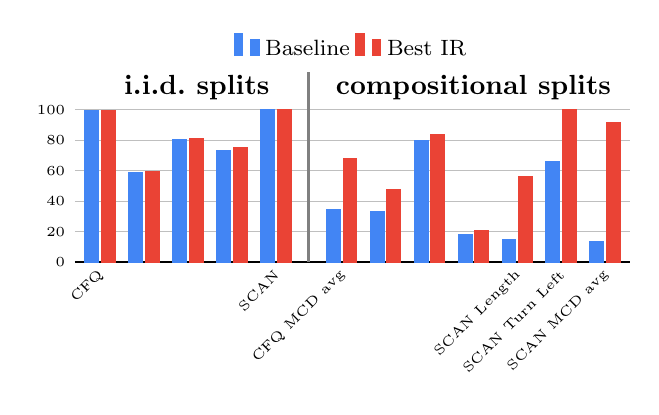
\begin{tikzpicture}
\begin{axis}[
    ybar=1pt,       height=10em,
    width=3.4in,
    bar width=5pt,
    enlarge x limits=0.05,  clip=false,     ymin=0, ymax=100,
    axis lines*=left,
    y axis line style={
        draw=none,
    },
    ymajorgrids=true,
xtick={
        0,1,2,3,4,
        5.5,6.5,7.5,8.5,9.5,10.5,11.5
    },
    xticklabels={
        CFQ,
        \atis{},
        \geo{},
        \scholar{},
        SCAN,
        CFQ MCD avg,
        \atis{},
        \geo{},
        \scholar{},
        SCAN Length,
        SCAN Turn Left,
        SCAN MCD avg,
    },
    xticklabel style={
        rotate=45,
        anchor=east,
        font=\tiny,
        xshift=4pt,
    },
    yticklabel style={
        font=\tiny,
    },
    tick style={draw=none},
legend style={
        legend columns=-1,
        at={(0.5,1.25)},
        anchor=south,
        draw=none,  font=\footnotesize,
    },
]
\draw[line width=1pt,gray]
    (axis cs: 4.75, 0) -- (axis cs: 4.75, 125);
\node[anchor=south]
    at (axis cs: 2.2, 100) {\textbf{i.i.d.\ splits}};
\node[anchor=south]
    at (axis cs: 8.5, 100) {\textbf{compositional splits}};
\addplot[draw=myblue,fill=myblue]
coordinates {
    (0, 99.5)
    (1, 58.6)
    (2, 80.6)
    (3, 72.9)
    (4, 100.0)
    (5.5, 34.6)
    (6.5, 32.9)
    (7.5, 79.7)
    (8.5, 18.1)
    (9.5, 14.5)
    (10.5, 66.1)
    (11.5, 13.4)
    };
\addplot[draw=myred,fill=myred]
coordinates {
    (0, 99.4)
    (1, 59.5)
    (2, 81.0)
    (3, 75.2)
    (4, 100.0)
    (5.5, 67.8)
    (6.5, 47.8)
    (7.5, 83.5)
    (8.5, 20.6)
    (9.5, 56.4)
    (10.5, 100.0)
    (11.5, 91.8)
    };
\legend{Baseline, Best IR}
\end{axis}
\end{tikzpicture}     \caption{Compared to Baseline (T5-base), the best IR of each split maintains the baseline accuracy for i.i.d.\ splits while giving large gains for compositional splits.}
    \label{fig:baseline_vs_ir_bar_chart}
\end{figure}

\subsection{Performance on i.i.d.\ Splits}

While our proposed IRs substantially improve the performance of T5 on compositional splits, we wish to verify they do not hurt performance on i.i.d.\ splits. To this end, we test our approaches with T5-base on the \emph{random} splits of \scan{} and \cfq{}, and on the standard i.i.d.\ splits of the text-to-SQL datasets.
As shown in Figure~\ref{fig:baseline_vs_ir_bar_chart} (see Table~\ref{tab:iid_results} for full results), we find that IRs indeed maintain the baseline accuracy on these i.i.d.\ splits.
%
